\begin{exercise}
      {ID-ceaa6860f9dc70886b1263597f896c56c2e89ceb}
      {Kreis und Dreieck}
  \ifproblem\problem
    \begin{minipage}{0.75\textwidth}
      Ein Kreis und ein Dreieck können einander auf verschiedene Arten
      schneiden. Im Folgenden sollen immer Punkte betrachtet werden, wo Kreis
      und Dreieck einander richtig schneiden und nicht nur berühren; in der
      Abbildung schneidet der Kreis das Dreieck zweimal und einmal berührt
      er das Dreieck.
    \end{minipage}\hfill
    \begin{minipage}{0.24\textwidth}
      \centering
      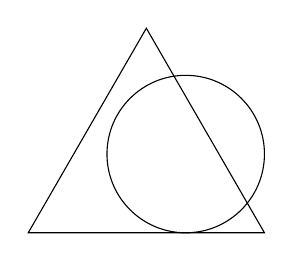
\begin{tikzpicture}
        \draw (0, 0) -- (0:3cm) -- (60:3cm) -- cycle;
        \draw (2, 1) circle (1cm);
      \end{tikzpicture}
    \end{minipage}\par
    \begin{enumerate}[a)]
      \item Zeichne einen Kreis und ein Dreieck, die einander genau zweimal
            schneiden und zwar so, dass die beiden Schnittpunkte auf derselben
            Dreiecksseite liegen.
      \item Zeichne einen Kreis und ein Dreieck, die einander genau zweimal
            schneiden und zwar so, dass die beiden Schnittpunkte auf verschiedenen
            Dreiecksseiten liegen.
      \item Zeichne einen Kreis und ein Dreieck, die einander genau viermal
            schneiden und zwar so, dass eine der Dreiecksseiten keinen Schnittpunkt
            aufweist.
      \item Zeichne einen Kreis und ein Dreieck, die einander genau viermal
            schneiden und zwar so, dass alle Dreiecksseiten vom Kreis geschnitten
            werden.
      \item Zeichne einen Kreis und ein Dreieck, die einander genau sechsmal
            schneiden.
    \end{enumerate}
  \fi
  %\ifoutline\outline
  %\fi
  %\ifoutcome\outcome
  %\fi
\end{exercise}
